\documentclass[letterpaper, 12pt]{article}
\usepackage[letterpaper, top=2.5cm, bottom=2.5cm, left=3cm, right=3cm]{geometry} %margenes
\usepackage[backend=biber]{biblatex}\addbibresource{referencias.bib}
\usepackage[utf8]{inputenc} %manejo de caracteres especiales
\usepackage[spanish]{babel} %manejo de encabezados de inglés a español
\usepackage{fancyhdr} %formato de los encabezados de página
\usepackage{ragged2e} %alineado real justficado
\usepackage{graphicx} %manejo de imagenes
\usepackage{amsmath} %manejo de notación matemática
\usepackage{mathtools} %manejo de notación matemática
\usepackage{blindtext} %texto de relleno
\usepackage{tikz} %manejo de diagramas electricos
\usepackage{circuitikz} %manejo de diagramas electricos
\usepackage{csquotes}
\usepackage[titles]{tocloft} %manejo de elementos para el índice
\usepackage{float} %manejo de centrado para figuras

\pagestyle{fancy}
\fancyhf{}
\rfoot{\thepage}

\nocite{*}

\begin{document}
    
    %PORTADA
    \begin{titlepage}
        \begin{figure}[ht]
            \centering
            
\includegraphics[width=15cm]{logosITT.png}
        \end{figure}
        \centering
        {\scshape\LARGE Tecnológico Nacional de México\\Instituto Tecnológico de Tijuana\par}
        \vspace{1cm}
        {\scshape\Large Princípios Electricos y Aplicaciones Digitales\par}
        \vspace{1cm}
        {\scshape\Large Unidad 1\par}
        \vspace{1.5cm}
        {\huge\bfseries Tarea 2\par}
        \vspace{2cm}
        {\Large\itshape Equipo D1N4Mic B00M\par}
        \vfill
        Profesor: \par
        Ing. Rigoberto Alvarado Rivera
        
        \vfill

        {\large 13 de noviembre del 2020}
    \end{titlepage}

    \newpage
    \thispagestyle{empty}
    \tableofcontents
    \listoffigures

    \newpage
    \begin{justify}
        \setcounter{page}{1}
        \thispagestyle{fancy}
        \lhead{\textbf{Tarea 2}}
        \rhead{\text{13 de noviembre del 2020}}

        \section{Tipos de diodos}
        \subsection{Láser}
        \subsubsection{Estructura}
        Dicho artefacto esta compuesto de las siguientes partes en órden (las cuales se pueden apreciar en la imagen \ref{fig:laser})
        \begin{itemize}
            \item Contacto metálico.
            \item Material tipo-P.
            \item Material tipo-N (región intrínseca).
            \item Material tipo-N.
            \item Contacto metálico.
        \end{itemize}
        \begin{figure}[H]
            \centering
            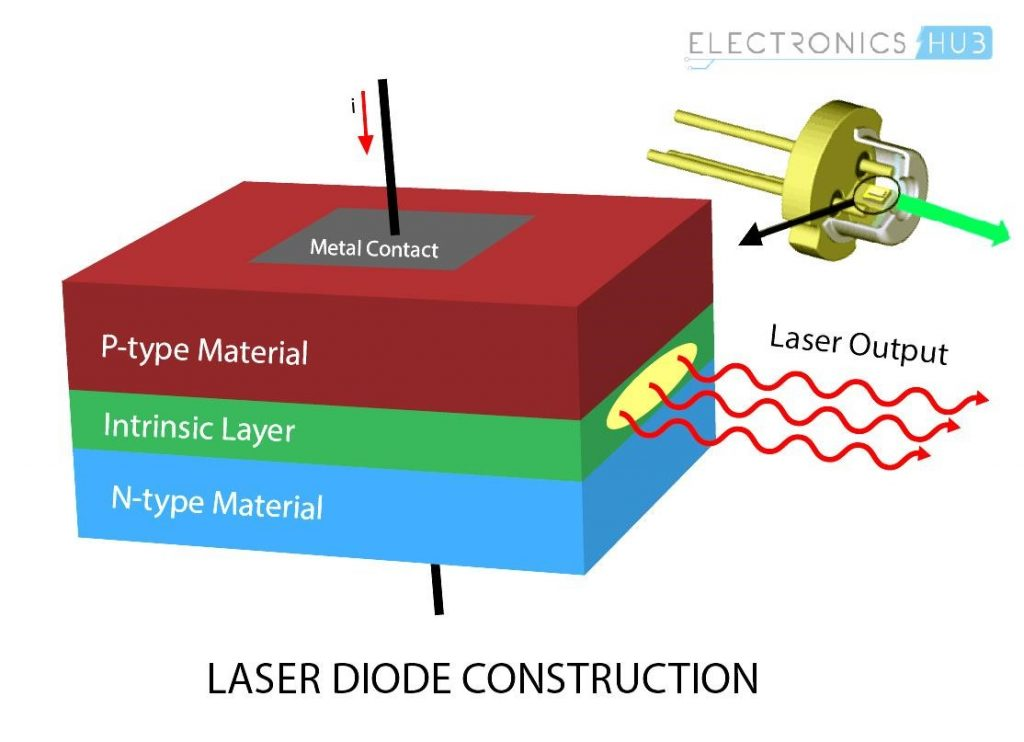
\includegraphics[width=10cm]{laserd.jpg}
            \caption{Modelo de la esctructura de un diodo láser.}
            \label{fig:laser}
        \end{figure}
        Las terminales de entrada están conectadas a unas placas metálicas las cuales hacen forma de un emparedado a las capas de tipo-P y tipo-N. La región intrínseca es usada para incrementar el volúmen de la región activa, para que un mayór numero de hoyos y electrónes
        se acumulen en la unión. Esto permite que un mayor número puedan re-combinarse con los hoyos en cualquier tiempo, resultando en una mejor salida de potencia. La luz láser es emitída desde la región elíptica. Este rayo del diódo puede ser enfocado más allá usando un lente
        óptico. Dicho arreglo normalmente está encerrado por una carcasa de
        \subsubsection{Funcionamiento}
        Para favorecer la emisión estimulada y generación de luz láser, el cristal semiconductor del diodo puede tener la forma de una lámina delgada con un lado totalmente reflectante y otro sólo reflectante de forma parcial,
        lográndose así una unión PN de grandes dimensiones con las caras exteriores perfectamente paralelas y reflectantes.\\\newline
        Este conjunto forma una guía de onda similar a un resonador de tipo Fabry-Perot. En ella, los fotones emitidos en la dirección adecuada se reflejarán repetidamente en dichas caras reflectantes, lo que ayuda a su vez a la emisión de más
        fotones estimulados dentro del material semiconductor y consiguientemente a que se amplifique la luz.
        \subsubsection{Aplicaciones}
        \begin{itemize}
            \item Lectores CD y DVD.
            \item Lectores de código de barras.
            \item Transmición de señal por cable y HDTV.
            \item Aplicaciones médicas incluyendo instrumentos quirúrgicos y para sanar la retina y el cerebro.
            \item Sistemas de detección de intrusos.
            \item Aplicaciones de control remoto.
            \item Aplicaciones industriales incluyendo soldadura, cortes de presición, tratamiento calorífico, etc.
            \item Comunicación de fibra óptica (usando varios tipos de cables de fibra óptica).
            \item Comunicación de alta velocidad a grandes distancias.
            \item Punteros láser.
            \item Impresión.
            \item Circuitos integrados.
            \item Sensación espectroscópica.
            \item Buscadores de rango.
        \end{itemize}
        \subsection{Fotodiódo}
        \subsubsection{Estructura}
        El fotodiódo estándar es basado en la unión PN. Sin empbargo, uno de los requerimientos clave de un fotodiódo es que tenga un área cómoda para recolectar la luz. Esto puede ser incrementado usando un diódo PIN, esto es debido a que el área intrínseca es incluida en la unión activa para recolección de la luz,
        lo que permite que exista una mayor area de recolección, haciendo que el fotodiódo PIN sea más efectivo. Se puede apreciar a mayor escala en la imágen siguiente
        \begin{figure}[H]
            \centering
            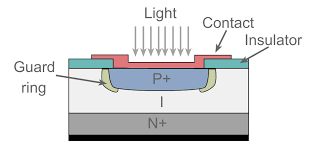
\includegraphics[width=8cm]{fdiodo.png}
            \caption{Modelo del fotodiódo tipo PN.}
            \label{fig:fdiodo}
        \end{figure}
        \subsubsection{Funcionamiento}
        El fotodiodo es polarizado inversamente permitiendo de esta manera el flujo de electrones o el flujo de la corriente en sentido inverso. Estos componentes tienen un lente que permite concentrar la luz que incide en ellos, por ello,
        cuando la luz que incide es de suficiente energía puede excitar un electrón generando movimiento y permitiendo la creación de huecos con carga positiva. Por lo tanto, entre mayor sea la intensidad de luz que incida en el fotodiodo mayor será
        la corriente que fluye.
        \subsubsection{Aplicaciones}
        \begin{itemize}
            \item Sensores de proximidad y detección remota.
            \item Control remoto.
            \item Lectores de código de barras.
            \item Lectores de CD y DVD.
            \item Fotometría y Espectrometría.
        \end{itemize}
        \subsection{Zener}
        \subsubsection{Estructura}
        Es una unión PN especial, muy dopada, diseñada para conducir en la dirección inversa cuando se alcanza un determinado voltaje especificado.
        \begin{figure}
            \centering
            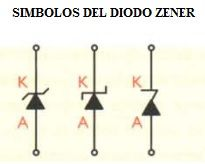
\includegraphics[width=10cm]{zener.jpg}
            \caption{Símbolo del diodo zener.}
            \label{fig:simzener}
        \end{figure}
        \subsubsection{Funcionamiento}
        Cuando polarizamos inversamente y llegamos al voltaje zenner el diodo conduce y mantiene la tensión de dicho voltaje constantante a pesar de que se aumente la tensión del circuito.
        Dicha corriente se le llama corriente inversa. Se le llama la zona de ruptura a por encima del voltaje zener. Antes de, el diodo no conduce.\\ \newline
        A grandes rasgos funciona como un regulador de voltaje.
        \subsubsection{Aplicaciones}
        \begin{itemize}
            \item Reguladores de tensión o de voltaje.
            \item Elementos protectores de circuitos.
            \item Recorte de de onda AC.
        \end{itemize}
        \subsection{Tunnel}
        \subsubsection{Estructura}
        Su estructura está construida por usar las dos terminales llamadas anódo y cátodo. El semiconductor tipo-P se comporta como el ánodo el material tipo-N actua como un cátodo.
        Algunos elementos usados para la encapsulación y manufactura son el germanio y el galio.
        \begin{figure}[H]
            \centering
            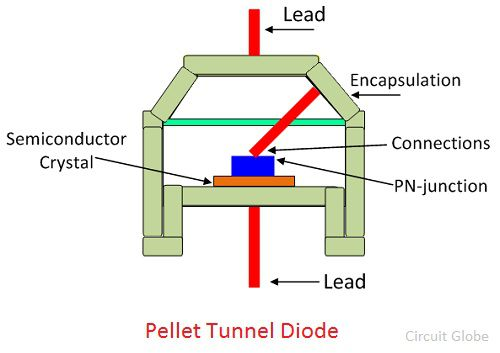
\includegraphics[width=10cm]{tunnel.jpg}
            \caption{Modelo del diodo Tunnel.}
            \label{fig:Dtunel}
        \end{figure}
        \subsubsection{Funcionamiento}
        Es un diodo semiconductor que tiene una unión PN, en la cual se produce el efecto tunel que le da el nombre al diodo. Esto da origen a una conductancia diferencial negativa
        en un cierto intervalo de la caraterística corriente-tensión. Cuando la resistencia es negativa, la corriente disminuye al aumentar el voltaje. 
        \subsubsection{Aplicaciones}
        \begin{itemize}
            \item Aplicaciones selectas como en circuitos osciladores de alta frecuencia.
        \end{itemize}
        
        \section{Transistores fototransistor, FET y MOSFET}
        \subsection{Fototransistór}
        \subsubsection{Estructura}
        Su estructura está específicamente optimizada para aplicaciones ópticas. Este contiene una base mas larga y areas recolectoras que pueden ser usadas en un transistor normal donde el contacto de emisión es comunmente desajustado entre la estructura. Esto asegura que una
        mayor cantidad de luz llegue a la región activa dentro del fototransistor. Los transistores mas modernos usan materiales semiconductores tipo III-V como arseniuro de galio.
        \begin{figure}[H]
            \centering
            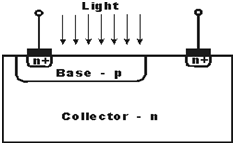
\includegraphics[width=8cm]{photo.png}
            \caption{Estructura de un fototransistor.}
            \label{fig:StructTransFoto}
        \end{figure}
        \subsubsection{Funcionamiento}
        Combinan en un mismo dispositivo la detección de luz y la ganancia. Su construcción es similar a la de los transistores convencionales, excepto que la superficie superior se expone a la luz 
        a través de una ventana o lente. Los fotones incidentes generan pares electrón-hueco en la proximidad de la gran unión CB. Las tensiones de polarización inversa de la unión CB, llevan los huecos
        a la superficie de la base y los electrones al colector. La unión BE polarizada directamente, hace que los huecos circulen de base a emisor mientras que los electrones fluyen del emisor a la base.
        \subsubsection{Aplicaciones}
        \begin{itemize}
            \item Aplicaciones de tipo ON-OFF.
            \item Sensor visual del ratón de computadora.
            \item Controles de iluminación.
            \item Lectores de cinta.
            \item Lápices ópticos
            \item Controles remotos.
        \end{itemize}
        \subsection{FET}
        \subsubsection{Estructura}
        Este transistor está formado por una barrita de material P ó N. llamada canal, rodeada en parte de su longitud por un collar del otro tipo de material que forma con el canal una unión P-N.
        En los extremos del canal se hacen sendas conexiones óhmicas llamadas respectivamente sumidero (d-drain) y fuente (s-source), más una conexión llamada puerta (g-gate) en el collar.
        \begin{figure}
            \centering
            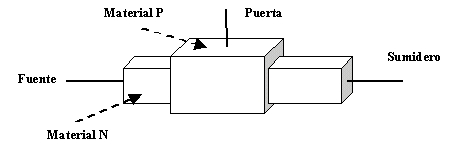
\includegraphics[width=10cm]{FET.jpg}
            \caption{Modelo de la estructura de un transistor FET.}
            \label{fig:FET}
        \end{figure}
        \subsubsection{Funcionamiento}
        La conducción tiene lugar gracias a ldesplazamiento de portadores de dos polaridades (huecos positivos y electrones negativos). Puesto que hay una tensión positiva en el drenador y el surtidor, los electrones fluirán desde el surtidor al drenador
        (o viceversa según la configuración del mismo), aunque hay que notar que también fluye una corriente despreciable entre el surtidor (o drenador) y la puerta, ya que el diodo formado por la unión canal-puerta, está polarizado inversamente.
        \subsubsection{Aplicaciones}
        \begin{itemize}
            \item Amplificador de poco ruido.
            \item Amplificador amortiguador.
            \item Amplificador Cascode.
            \item Interruptor analógico.
            \item Cortador.
            \item \emph{Multiplexer.}
            \item Limitador de corriente.
            \item Osciladores de cambio de fase.
        \end{itemize}
        \subsection{MOSFET}
        \subsubsection{Estructura}
        Es un transistor unipolar que tiene tres terminales las cuales son la fuente, el portón y el drenaje. Aparte de estas, está un sustrato llamado el cuerpo el cual está siempre
        conectado a la terminal fuente. Es fabricado por la oxidación de sustratos de silicón.
        \begin{figure}
            \centering
            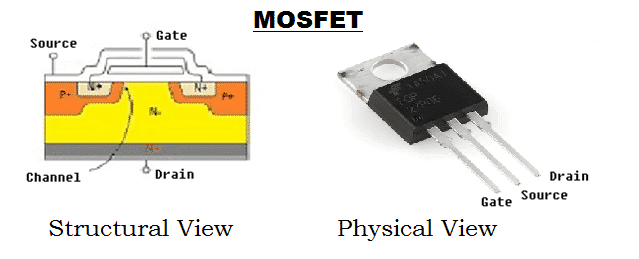
\includegraphics[width=10cm]{MOSFET.png}
            \caption{Vista estructural y física de un transistor MOSFET.}
        \end{figure}
        \subsubsection{Funcionamiento}
        Su funcionamiento a grandes rasgos es causado por la alteración de la longitud del canal por el cual el movimiento de transportadores de carga (electrones del canal-N y los hoyos del canal-P) ocurre desde
        la fuente hasta el drenaje. El terminal portón es insulado, y de su voltaje se regula la conductividad del dispositivo.
        \subsubsection{Aplicaciones}
        \begin{itemize}
            \item Interruptor.
            \item Control automático del alumbrado público.
            \item Control de velocidad pre-establecida de un motór BLCD
            \item Ahorrador de energía para alumbrado público controlado por intensidad.
            \item etc.
        \end{itemize}
        \section{\emph{Opto-isolator}}
        \subsection{¿Qué es?}
        Conocido también como \emph{Optocoupler} (Acoplador óptico). Es un dispositivo eletrónico que tranfiere la energía eléctrica de un circuito a otro
        por medio de un camino de transmisión óptica mientras provee aislamiento eléctrico entre los dos circuitos. Este acopla voltajes altos de un lado a otro sin ningún contacto
        eléctrico.\\
        De manera más detallada, el Octocoupler convierte la energía eléctrica en un rayo de luz usando un diodo emitidor de luz, y despues redirecciona dicha luz hacia el sensor óptico como lo puede ser
        un fotodiódo o un fototransistor, los cuales convierten la energía óptica a energía eléctrica. Esto aísla a los dos circuitos, prevee subidas repentinas de voltaje, y disminuye el ruido y la interferencia
        asociadas con las conexiónes de comunicación. Esto se puede apreciar en la siguiente imágen (figura \ref{fig:Optothingy}). 
        \begin{figure}[H]
            \centering
            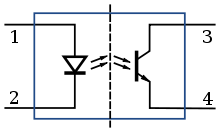
\includegraphics[width=8cm]{Optothingy.png}
            \caption{Ejemplo de diagrama eléctrico de un Optocoupler.}
            \label{fig:Optothingy}
        \end{figure}
        \subsection{¿Para qué se utiliza?}
        En general, este dispositivo es muy usado en distintas aplicaciones ópticas incluyendo suministros de energía para proveer insolación, en la industria de grabaciones para reducír interferencia, y en sistemas computacionales
        para tranferencia de datos. Otras incluyen:
        \begin{itemize}
            \item Sistemas de retroalimentación de fuente de alimentación.
            \item Aplicaciones médicas e industriales.
            \item Aislamiento de corrientes buclé de tierra.
            \item Transición de niveles altos de voltaje.
            \item Aislamiento de señales.
            \item Aislamiento de potencia eléctrica y de ruido.
        \end{itemize}

        \section{SSD \emph{Solid-state Device}}
        \subsection{Proceso de manufactura}
        Dichas unidades usan chips de memoria flash para almacenar información, por ende un SSD se fabrica de muchos chips de memoria instalados en el tablero del circuito. La distribuidora más grande de la cual se ba a basar la explicación
        del proceso de manufactura es la de la compañia Micron.
        \\\newline
        Se utilizan wafers de silicona los cuales son manejados por una linea de producción para evitar contaminación de los mismos. A medida que estos se mueven en la linea de producción, se le agregan distintas capas de otros materiales, incluyendo conductores
        como el cobre, y materiales no conductivos, como el dióxido de silicona. Después de que se aplica cada capa de material, el wafer se recubre con fluido sensible a la luz. Luego, se le aplica luz ultravioleta mediante un esténcil de vidrio del patrón de circuito eléctrico.
        Cuando la luz entra en contacto con los materiales, estos se rompen y disuelven. Cuando los materiales permanecen protegidos por el esténcil, se conservan intactos, lo que imprime el patrón del circuito en el wafer. Entonces los baños químicos eliminan cualquier material residual.
        \\\newline
        Después de la impresión, cada wafer de 30 centímetros contiene cientos de chips, que deben permanecer separados. Después de que los chips se cortan por separado, se insertan en una carcasa de plástico protector.
        \\\newline
        Los tableros de circuitos grandes se cubren con pasta de soldadura de aleación de estaño en las áreas donde se fijarán los chips de memoria y otros componentes. Un robot fija los componentes al tablero, luego los tableros montados pasarán a un horno en el que se fusionan con los componentes.
        \begin{figure}[H]
            \centering
            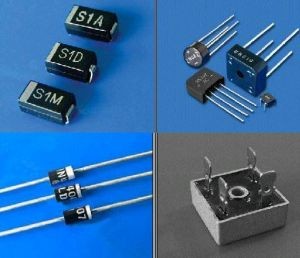
\includegraphics[width=10cm]{ssd.jpg}
            \caption{Ejemplos varios de SSD's.}
            \label{fig:SSDS}
        \end{figure}
        \subsection{Ventajas}
        \begin{itemize}
            \item Son compactos, menos espacio se traduce a más dispositivos.
            \item Sus capacidades como semiconductores, los hace eficientes en circuitos.
            \item Permite usarlos en electrónica digital.
        \end{itemize}
        \subsection{Aplicaciones}
        \begin{itemize}
            \item Circuitos integrados.
            \item Transistores en radios y amplificadores.
            \item Memorias y Almacenamiento digital.
            \item Luces.
        \end{itemize}
        \section{Funcionamiento de las computadoras analógicas}
        A grandes rasgos, las computadoras analógicas funcionan de la siguiente manera: las entradas se convierten en tensiones que pueden sumarse o multiplicarse empleando elementos de circuito de diseño especial. Las respuestas se generan continuamente para su visualización o para
        su conversión en otra forma deseada. Basicamente está orientada a resolver ecuaciones diferenciales ordinarias. Esto le permite simular modelos de sistemas dinámicos. Tambiéen opera mediante la generación de voltajes que se comportan como lo hacen las variables físicas o matemáticas
        en el sistema en estudio. Cada variable se representa por una señal en forma de voltaje continuamente variable, a la salida de una unidad programada de cálculo.
        \begin{figure}[H]
            \centering
            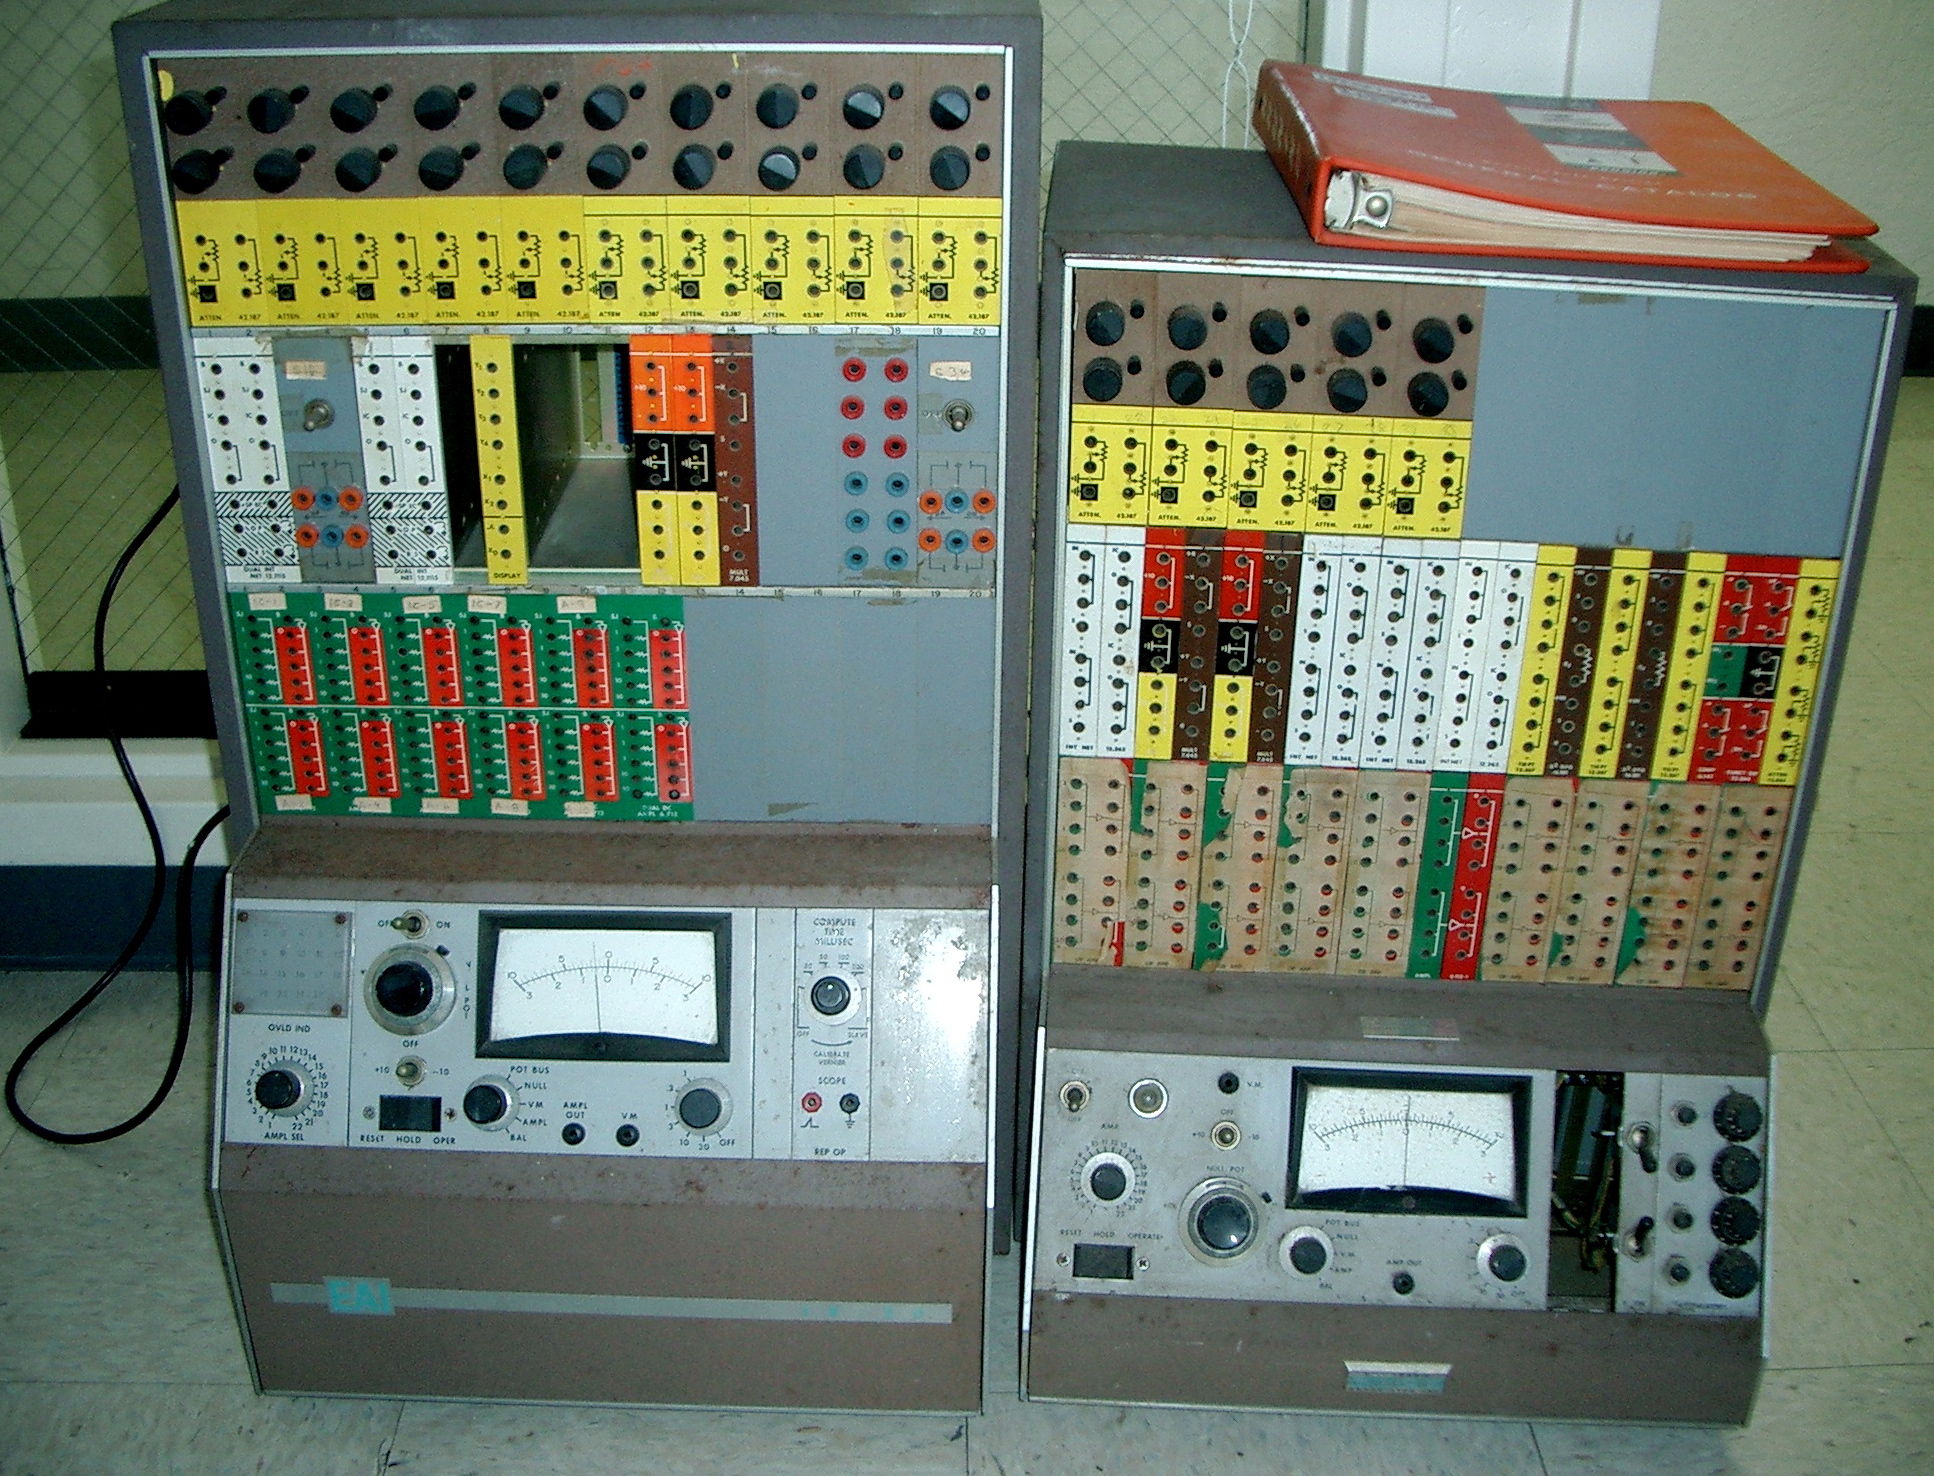
\includegraphics[width=10cm]{analog.jpg}
            \caption{Ejemplo de una computadora analógica}
            \label{fig:analog}
        \end{figure}
        \section{Tubos de vacío}
        Conocido también como válvulas de vacío. Es un diódo desarrollado por el físico inglés John Ambrose Fleming. Se atribuye al invertor neoyorquino Lee de Forest en 1907 a la patente del Triodo.
        \\
        Este a grandes rasgos contiene dos electrodos, el cátodo el cual es un filamento caliente o un pequeño tubo de metal caliente ue emite electrones a través de emisión termoiónica, y el ánodo, una placa que es el elemento colector de electrones. En los diódos
        los electrones emitidos por el cátodo son atraídos por la placa sólo cuando ésta es positiva con respecto al cátodo. Cuando la placa está cargada negativamente, no circula por el tubo. Si se aplica un potencial alterno a la placa, la corriente pasará por el 
        tubo solamente durante la mitad positíva del ciclo, actuando como rectificador.
        \begin{figure}[H]
            \centering
            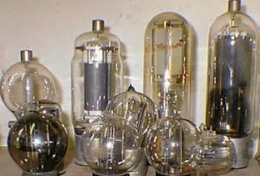
\includegraphics[width=8cm]{tubitos.jpeg}
            \caption{Tubos de vacío varios}
            \label{fig:tubitos}
        \end{figure}

        \section{CRT (Cathode-ray tube)}
        Conocido por el nombre completo en español \emph{(tubo de rayos catódicos)}. Es un tubo de vacío de vidrio dentro de los cuales un cañón de electrones emite una corriente de electrones guiadas por un campo eléctrico hacia una pantalla cubierta de pequeños elementos
        fosforecentes. Está compuesto por un cátodo, un electrodo metálico con carga negativa, y uno o más ánodos (electrodos con carga positiva). El cátodo emite los electroens atraídos por el ánodo. El ánodo actúa como un acelerador y concentrador de los electrones, creando
        una corriente de electrones dirigida a la pantalla. Un campo magnético va guiando los electrones dirigída a la pantalla. Un campo magnético va guiando los electrones de derecha a izquierda y de arriba hacia abajo. Se crea con dos placas electrificadas X e Y (llamadas deflectores)
        que envían la corriente en dirección horizontal y vertical, respectivamente.
        \begin{figure}[H]
            \centering
            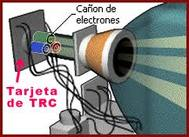
\includegraphics[width=6cm]{ctr.jpeg}
            \caption{Principio de funcionamiento del tubo de rayos catódicos}
            \label{fig:ctr}
        \end{figure}
        \section{Amplificador diferencial}
        \subsection{Idea de funcionamiento}
        A grandes rasgos, el amplificador más básico tiene 2 entradas \(V_1\) y \(V_2\). Si la tensión de \(V_1\) aumenta, la corriente del emisor del transistor \(Q_1\) aumenta,
        causando una caída de tensión en \(R_e\). Si la tensión de \(V_2\) se mantiene constante, la tensión entre base y emisor del transistor \(Q_2\) disminuye, reduciéndose también la corriente
        de emisor del mismo transistor. Esto causa que la tensión de colector de \(Q_2\) aumente. La entrada \(V_1\) es la entrada no inversora de un amlificador operacional. Del mismo modo cuando la tensión
        en \(V_2\) aumenta, también aumenta la corriente de colector del transistor \(Q_2\), causando que la tensión de colector del mismo transistor disminuya. La entrada \(V_2\) es la entrada inversora del amplificador
        operacional. Si el valor de la resistencia \(R_E\) fuera muy grande, obligaría a la suma de las corrientes de emisor de los transistor \(Q_1\) y \(Q_2\), a mantenerse constante, comportándose como una fuente de corriente.
        Entonces, al aumentar la corriente de colector de un transistor, disminuirá la corriente de colector del otro transistor. Por eso cuando la tensión \(V_1\) crece, la tensión en \(V_2\) decrece.
        \begin{figure}[H]
            \centering
            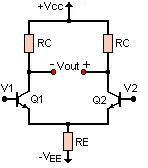
\includegraphics[width=6cm]{dxamp.jpg}
            \caption{Circuito de un Amplificador Diferencial.}
            \label{fig:dxamp}
        \end{figure}
        \subsection{Relación con el diferencial usado en una transmisión automotríz}
        \begin{itemize}
            \item La estructura básica es similar.
            \item El principio de funcionamiento es similar.
            \item Su planteamiento matemático es prácticamente el mismo.
        \end{itemize}
    \end{justify}
     
    \newpage
    \addcontentsline{toc}{section}{Referencias}
    \printbibliography

\end{document}